% !TeX root = ../main.tex

\section{RQ2: Interaction Complexity Analysis}
\vspace{-3pt}
\subsection{Methodology}

The workflow in Fig.~\ref{overview_fig} only shows the general~flow~among different modules. The details of interactions among components are still uncovered. We consider the interaction among two or more components, with at least one ML component.
An interaction pattern contains a module placeholder, which could be instantiated with components in the module~to~generate~interaction instances.
For example, pattern (PolicyEnsemble, [Policy]) could be instantiated as (PolicyEnsemble, TEDPolicy) or (PolicyEnsemble, (TEDPolicy, RulePolicy)). To answer \textbf{RQ2}, we conducted a qualitative and quantitative analysis of the component interaction patterns and instances of components.

\textbf{Step 1: Extract interaction patterns.}
The interaction can be divided into two categories: inter-module interaction and intra-module interaction.
(1) Inter-module interaction: the interaction between two adjacent modules (e.g., Featurizer with Tokenizer) was considered. We analyzed the usages~of~\texttt{Message} in the component code, as components use the \texttt{Message} class to transfer data. Specifically, we extracted all interaction patterns of its upstream and downstream components. We also considered the interaction between post-processing components (i.e., \textit{FallbackClassifier}, \textit{EntitySynonymMapper} and \textit{PolicyEnsemble}) and other components in their residing modules as inter-module interaction.
(2) Intra-module interaction: we identified interaction patterns for components within each module.

\textbf{Step 2: Generate interaction instances.}
For each inter-module interaction pattern, we instantiated the module placeholder with every component in the module. 
For every intra-module interaction, we derived the Cartesian product~of~all components in each module as interaction instances.
We~then filtered out component instances that do not contain ML~components, or do not meet the constraints specified~in~Rasa~documentation. 
For example, \textit{CRFEntityExtractor} could not use features of \textit{SparseFeaturizer} other than \textit{RegexFeaturizer}.
% For example, \textit{PolicyEnsemble} could interagete one, two or more Policies.

\textbf{Step 3: Summarize the interaction taxonomy.} For generated component patterns and instances, we analyzed their semantics and summarized a component interaction taxonomy.

\subsection{Results}
\begin{figure}[!t]
    \centering
    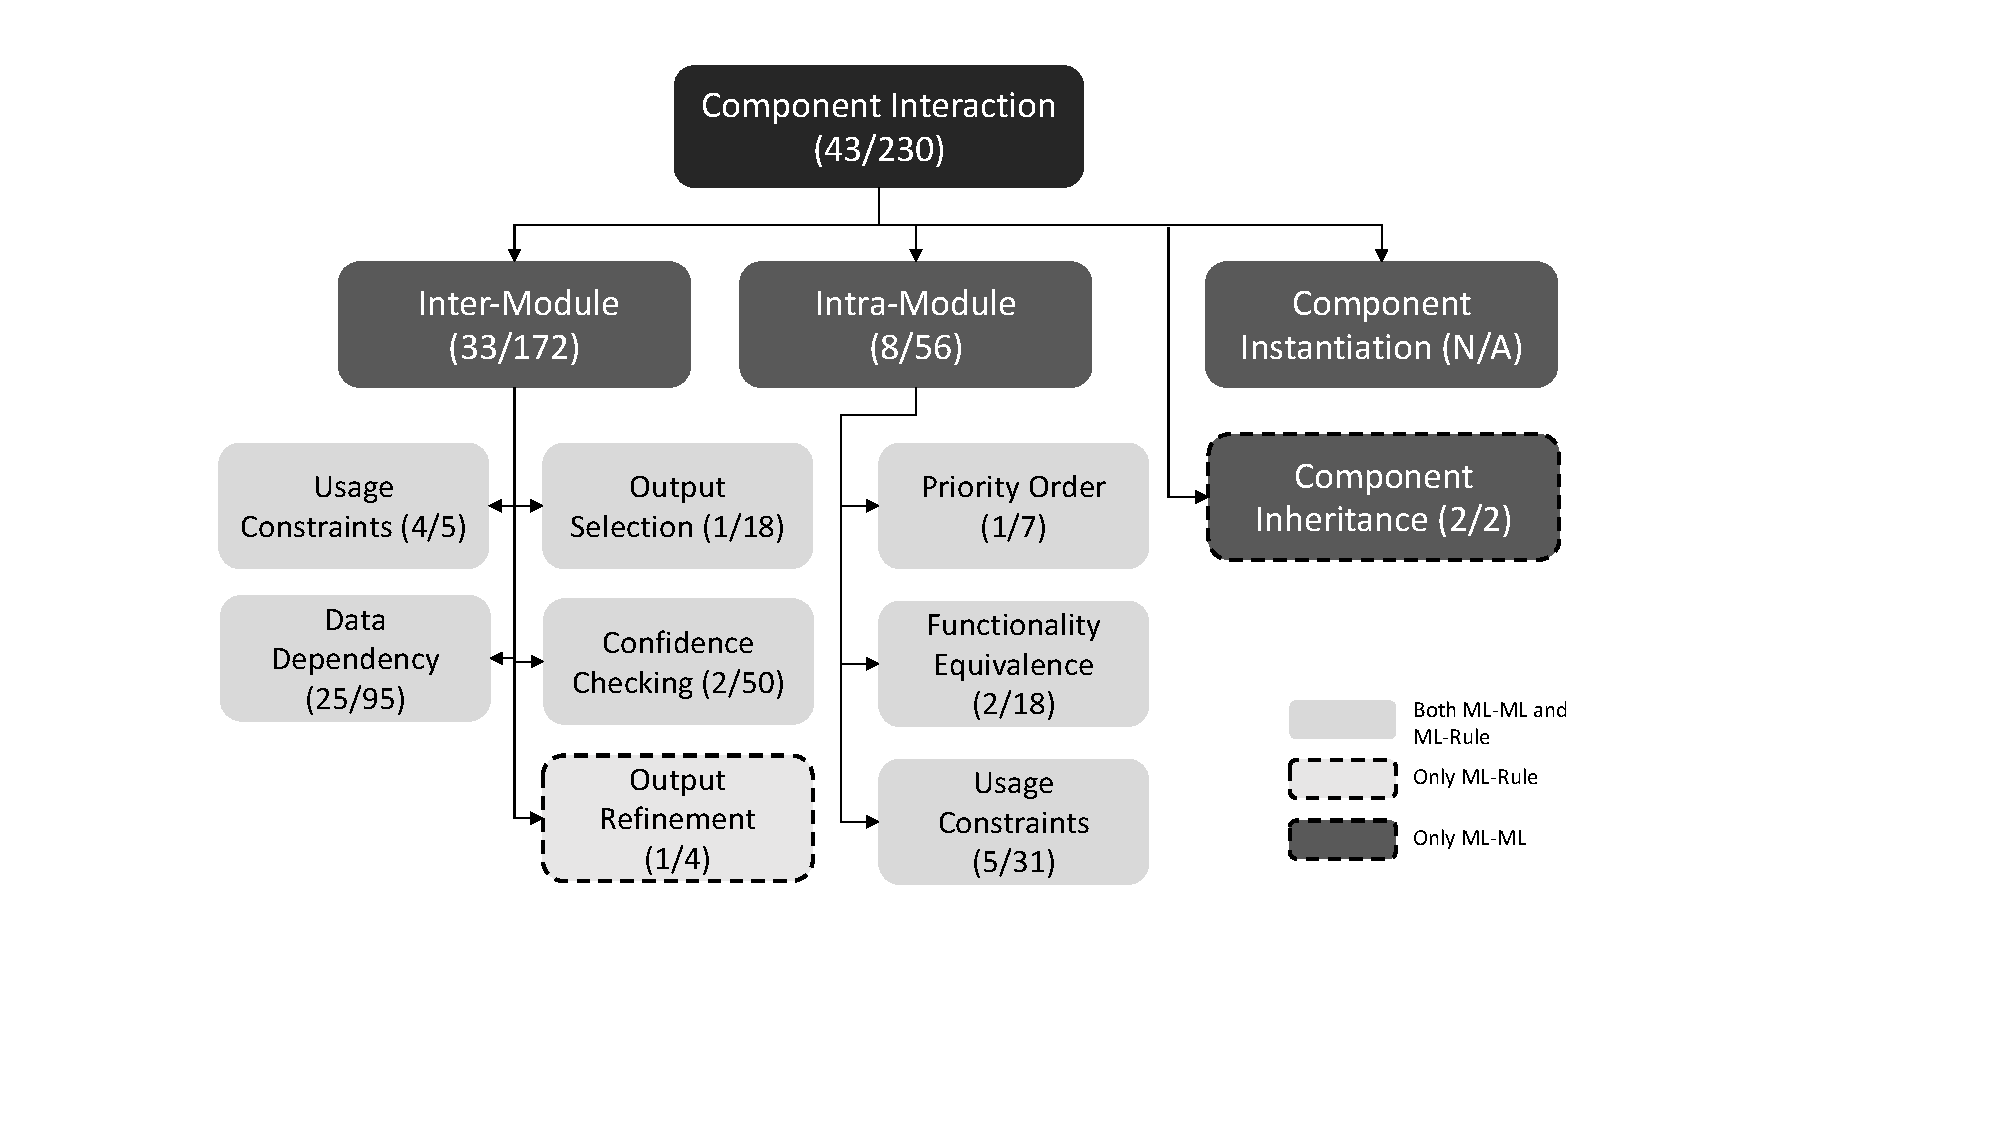
\includegraphics[scale=0.38]{figs/component_interaction.pdf}
    \caption{Taxonomy of Component Interactions}
    \label{component_interaction_fig}
\end{figure}

The component interaction taxonomy is shown in Fig. \ref{component_interaction_fig}. It is divided into 4 high-level categories (i.e. \textit{Inter-Module}, \textit{Intra-Module}, \textit{Component Instantiation} and \textit{Component Inheritance}) and 8 inner categories. 
Note that only \textit{Inter-Module} interactions contain components with direct data dependencies, while other categories contain components with indirect interactions (e.g., two featurizers are used together). The number of interaction patterns and interaction instances in each category~is~listed~as \textit{pattern\_count}/\textit{instance\_count} in Fig. \ref{component_interaction_fig}. There are a total of 43 interaction patterns and 230 interaction instances.
Nearly all categories include both ML to ML components and ML to rule-based components interactions. On the contrary, previous work on Apollo \cite{pengFirstLookIntegration2020} also presented 4 of the 8 inner categories, but did not provide a taxonomy and quantitative analysis. 

% \todo{Question: whther add number propertion of each category?}
% \todo{2 types of interaction covered in Apollo analysis.}

\textbf{Inter-Module}. Components from multiple modules interact through data transfers. In particular, \textit{Output Selection} means that the downstream component selects the proper output from multiple upstream outputs based on configurable criteria, e.g., \textit{PolicyEnsemble} with policies. 
\textit{Output Refinement} denotes that the downstream component complements the imperfect outputs of upstream components with rules, e.g., 
\textit{EntitySynonymMapper} with entity extractors. \textit{Confidence Checking} means that the downstream component checks reliability of the output from upstream components using ML models (e.g., \textit{UnexpecTEDIntentPolicy} with intent classifiers) or rules (e.g., \textit{FallbackClassifier} with IntentClassifiers). If the outputs are marked as not reliable, fallback behaviors such as the \texttt{fall\_back} system action are triggered. 
% \todo{Question: these compoenets are in the same module in Table I. and the functionability of them have been described in RQ1}.
\textit{Usage Constraints} defines components that should or should not be used together under certain circumstances. For example, \textit{SpacyTokenizer} is required by \textit{CountVectorsFeaturizer} when applying \texttt{use\_lemma} option and \textit{LexicalSyntacticFeaturizer} when applying \texttt{pos\_tag} option. \textit{Data Dependency} includes the rest of inter-module interaction patterns that do not fall into any of the above categories, which are relatively ``trivial" interactions with no specific semantics.

\textbf{Intra-Module}. The interaction mode of components within a module differs from \textbf{Inter-Module}. These components interact indirectly when used together. 
\textit{Priority Order} means that the outputs of components within a module are selected according to priority order, e.g., the priority order of policies.
\textit{Usage Constraints} is similar to \textit{Usage Constraints} in the inter-module category. For example, only one component in any of \textit{Tokenizer}, \textit{IntentClassifier} and \textit{EntityExtractor} should be used in each configuration file, otherwise outputs of additional components will be overwritten.  \textit{Functionality Equivalence} includes all intra-module interaction patterns that do not belong to any of the above categories, which are relatively ``trivial" interactions involving components used together with no specific semantics.

\textbf{Component Instantiation}. Rasa supports creating multiple instances of a component within a configuration setting. For example, multiple \textit{CountVectorFeaturizers} instances with different ngram settings, and multiple \textit{LanguageModelFeaturizer} instances with different language models could be used together. We did not count this category of interaction patterns and instances, since developers could specify infinite instances of a component within a configuration setting.

\textbf{Component Inheritance}. The class inheritance mechanism allows ML models to be shared among components. For example, ML model definition class  in \textit{UnexpecTEDIntentPolicy} is a subclass of the ML model definition class in \textit{TEDPolicy}.

\subsection{Implications}

%Our results reflect that the interaction complexity of Rasa are from the following aspects.

\textbf{Lack of specifications for interactions.} The outputs of ML components for specific inputs are not guaranteed due to the stochastic nature of ML models  \cite{feature_interaction}. Thus, formulating interaction semantics in ML-enabled systems is more challenging than in traditional systems. When testing samples are predicated incorrectly, localizing the exact faulty component becomes difficult. 
Moreover, even if the faulty component has been fixed and performance of it has been improved, the overall performance of the entire system may degrade \cite{fix_that_fails}. Consequently, training and evaluation should be extended from component-level to system-level to consider interactions among components. 
In summary, we need to pay more attention to addressing the challenges caused by the lack of specifications in bug localization and repairing for ML-enabled systems.

\textbf{Hidden interactions}. Identifying all interactions is non-trivial, even for Rasa system developers. 
% Specifically, components inside one module may depend on different upstream components. 
For example,~the \textit{Data Dependency} interaction between \textit{RegexFeaturizer} and \textit{CRFEntityExtractor} is documented and can only be identified through source code analysis.
Application developers may misuse components and get confused with the poor~performance of the system without understanding the hidden~interactions, especially for interaction categories like \textit{Usage Constraints}, \textit{Output Selection} and \textit{Priority Order}.
Techniques like~data flow analysis can be explored to automatically reveal component interactions in ML-enabled systems \cite{Sattler2017LiftingID}.

Furthermore, our results on component interaction complexity could be helpful to guide developers to build~better~ML-enabled systems.
For example, developers can follow interaction patterns \textit{Output Selection} and \textit{Output Refinement} to improve the outputs of components at system level, as well as utilizing  \textit{Confidence Checking} to detect cases that ML models~can~not handle, and then triggering fallback rules, which is very important in safety-critical systems like self-driving systems~\cite{pengFirstLookIntegration2020}.


% \textbf{Complexity from code/model resue. } 

% \textbf{Complexity from huge interaction instances.} 
% not all interactions could be covered in configuration file, test coverage.
% hard to evaluate the performance under different interactions (developer may specifity)
